\clearpage
\subsection{MSVC + \olly}
\index{\olly}

\RU{Попробуем этот же пример в}\EN{Let's try this example in} \olly.
\RU{Загружаем, нажимаем F8 (\stepover) до тех пор, пока не окажемся в своем исполняемом файле,
а не в}\EN{Let's load it, press F8 (\stepover) until we get into our executable file
instead of} \TT{ntdll.dll}.
\RU{Скроллим вверх, до тех пока не найдем \main}\EN{Scroll up until \main appears}.
\RU{Кликаем на первой инструкции}\EN{Let's click on the first instruction} (\TT{PUSH EBP}), 
\RU{нажимаем}\EN{press} F2, \RU{затем}\EN{then} F9 (Run) \RU{и брякпойнт срабатывает
на начале \main}\EN{and a breakpoint will trigger when \main begins}.

\RU{Трассируем до того места, где готовится адрес переменной $x$}
\EN{Let's trace to the place where the address of variable $x$ is prepared}:

\begin{figure}[H]
\centering
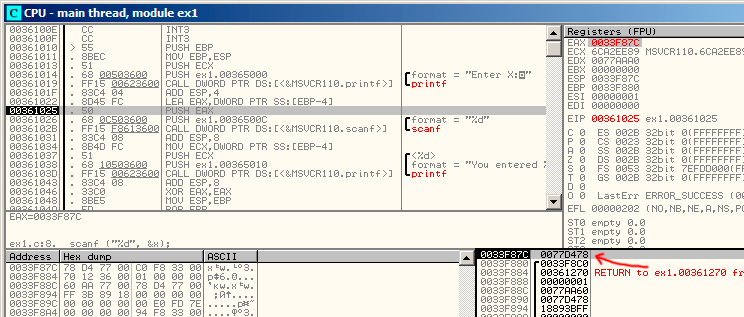
\includegraphics[scale=\FigScale]{patterns/04_scanf/1_simple/ex1_olly_1.png}
\caption{\olly: \RU{вычисляется адрес локальной переменной}\EN{address of the local variable is computed}}
\label{fig:scanf_ex1_olly_1}
\end{figure}

\RU{На \EAX в окне регистров можно нажать правой кнопкой и далее}
\EN{It is possible to right-click on \EAX in the registers window and then} ``Follow in stack''.
\RU{Этот адрес покажется в окне стека}\EN{This address will appear in the stack window}.
\RU{Смотрите, это переменная в локальном стеке}\EN{Look, this is a variable in the local stack}.
\RU{Я нарисовал там красную стрелку}\EN{I drew a red arrow there}.
\RU{И там сейчас какой-то мусор}\EN{And there is some garbage} (\TT{0x6E494714}).
\RU{Адрес этого элемента стека сейчас, при помощи \PUSH, запишется в этот же стек, рядом}
\EN{Now the address of the stack element with the help of \PUSH will be written to the same stack, next to it}.
\RU{Трассируем при помощи F8 вплоть до конца исполнения \scanf}\EN{Let's trace with F8 until the execution of \scanf finishes}.
\RU{А пока \scanf исполняется, в консольном окне, вводим, например, 123}
\EN{During the moment of \scanf execution, we enter, for example, 123, in the console window}:

\begin{figure}[H]
\centering
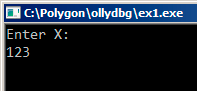
\includegraphics[scale=\NormalScale]{patterns/04_scanf/1_simple/ex1_olly_2.png}
\caption{\RU{Вывод в консоль}\EN{Console output}}
\label{fig:scanf_ex1_olly_2}
\end{figure}

\clearpage
\RU{Вот тут }\scanf \RU{отработал}\EN{executed here}:

\begin{figure}[H]
\centering
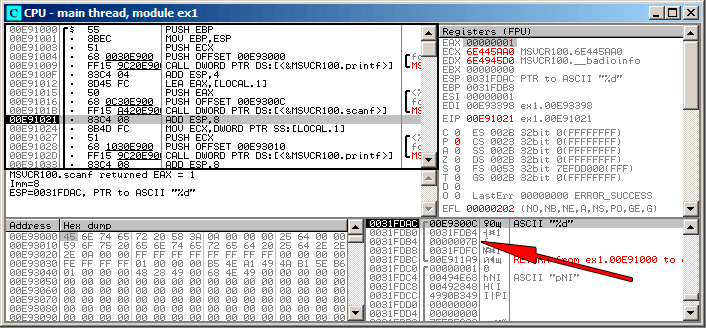
\includegraphics[scale=\FigScale]{patterns/04_scanf/1_simple/ex1_olly_3.png}
\caption{\olly: \scanf \RU{исполнилась}\EN{executed}}
\label{fig:scanf_ex1_olly_3}
\end{figure}

\scanf \RU{вернул}\EN{returns} $1$ \InENRU \EAX, \RU{что означает, что он успешно прочитал одно 
значение}\EN{which means that it has read one value successfully}.
\RU{В наблюдаемом нами элементе стека теперь}\EN{The element of 
stack we are looking at now contains} \TT{0x7B} (123).

\clearpage
\RU{Чуть позже, это значение копируется из стека в регистр \ECX и передается в \printf}
\EN{Further, this value is copied from the stack to the \ECX register and passed to \printf}:

\begin{figure}[H]
\centering
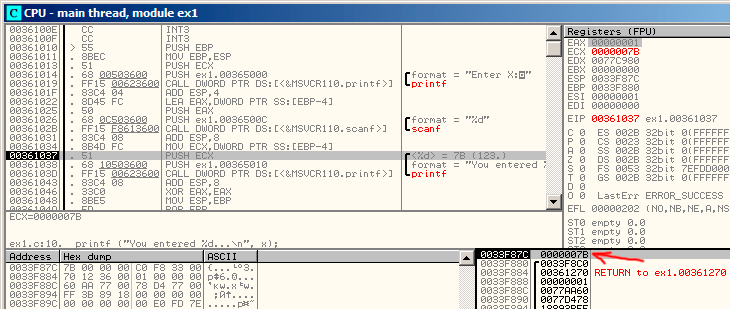
\includegraphics[scale=\FigScale]{patterns/04_scanf/1_simple/ex1_olly_4.png}
\caption{\olly: \RU{готовим значение для передачи в}\EN{preparing the value for passing into} \printf}
\label{fig:scanf_ex1_olly_4}
\end{figure}
